\documentclass[11pt, oneside]{scrartcl}   	% use "amsart" instead of "article" for AMSLaTeX format
\usepackage[top=2cm,right=2cm,bottom=2.5cm,left=2cm]{geometry}                		% See geometry.pdf to learn the layout options. There are lots.
% \usepackage[top=4cm,right=4cm,bottom=4cm,left=4cm]{geometry}
\geometry{letterpaper}                   		% ... or a4paper or a5paper or ... 
%\geometry{landscape}                		% Activate for for rotated page geometry
%\usepackage[parfill]{parskip}    		% Activate to begin paragraphs with an empty line rather than an indent
\usepackage[parfill]{parskip}
\usepackage{graphicx}				% Use pdf, png, jpg, or eps§ with pdflatex; use eps in DVI mode
								% TeX will automatically convert eps --> pdf in pdflatex
\usepackage{amssymb}
\usepackage{amsmath}

\usepackage[TS1,T1]{fontenc}
%\usepackage{fourier, heuristica}
\usepackage{array, booktabs}
\usepackage[x11names]{xcolor}
\usepackage{colortbl}
\usepackage{caption}
\usepackage{bbm}
\usepackage{amssymb}
\usepackage{amsmath}
\usepackage{subfigure}
\DeclareCaptionFont{blue}{\color{LightSteelBlue3}}

\newcommand{\foo}{\color{LightSteelBlue3}\makebox[0pt]{\textbullet}\hskip-0.5pt\vrule width 1pt\hspace{\labelsep}}

\definecolor{light-gray}{gray}{0.7}

\title{Results}
\author{Joseph Boyd}
% \date{}							% Activate to display a given date or no date

\begin{document}

\maketitle

\tableofcontents

\section{Baseline}
\subsection{Header model - Cora dataset}
\subsection{Header model - Cora dataset appending HEP dataset}
\subsection{Header model - Cora and HEP combined datasets}
\subsection{Header model - HEP dataset}
\subsection{Header model - HEP dataset appending CORA dataset}
\subsection{Header model - HEP dataset appending 1/3 CORA dataset}
\subsection{Header model - HEP dataset appending 2/3 CORA dataset}
\subsection{Segmentation model - Cora dataset}
\subsection{Segmentation model - Cora dataset appending HEP dataset}
\subsection{Segmentation model - Cora and HEP combined datasets}
\subsection{Segmentation model - HEP dataset}
\subsection{Segmentation model - HEP dataset appending CORA dataset}

\section{Regularisation}
\subsection{Header model - $L2 = 0$}
\subsection{Header model - $L2 = 1e^{-6}$}
\subsection{Header model - $L2 = 1e^{-5}$}
\subsection{Header model - $L2 = 1e^{-4}$}
\subsection{Header model - $L2 = 1e^{-3}$}

\section{Dictionaries}
\subsection{Header model - HEP dataset}
\subsection{Header model - HEP dataset appending CORA dataset}
\subsection{Segmentation model - HEP dataset}
\subsection{Segmentation model - HEP dataset appending CORA dataset}

\section{Dictionaries + stop words}
\subsection{Header model - HEP dataset}
\subsection{Header model - HEP dataset appending CORA dataset}
\subsection{Segmentation model - HEP dataset}
\subsection{Segmentation model - HEP dataset appending CORA dataset}

%\begin{figure}[!ht]
%\center
%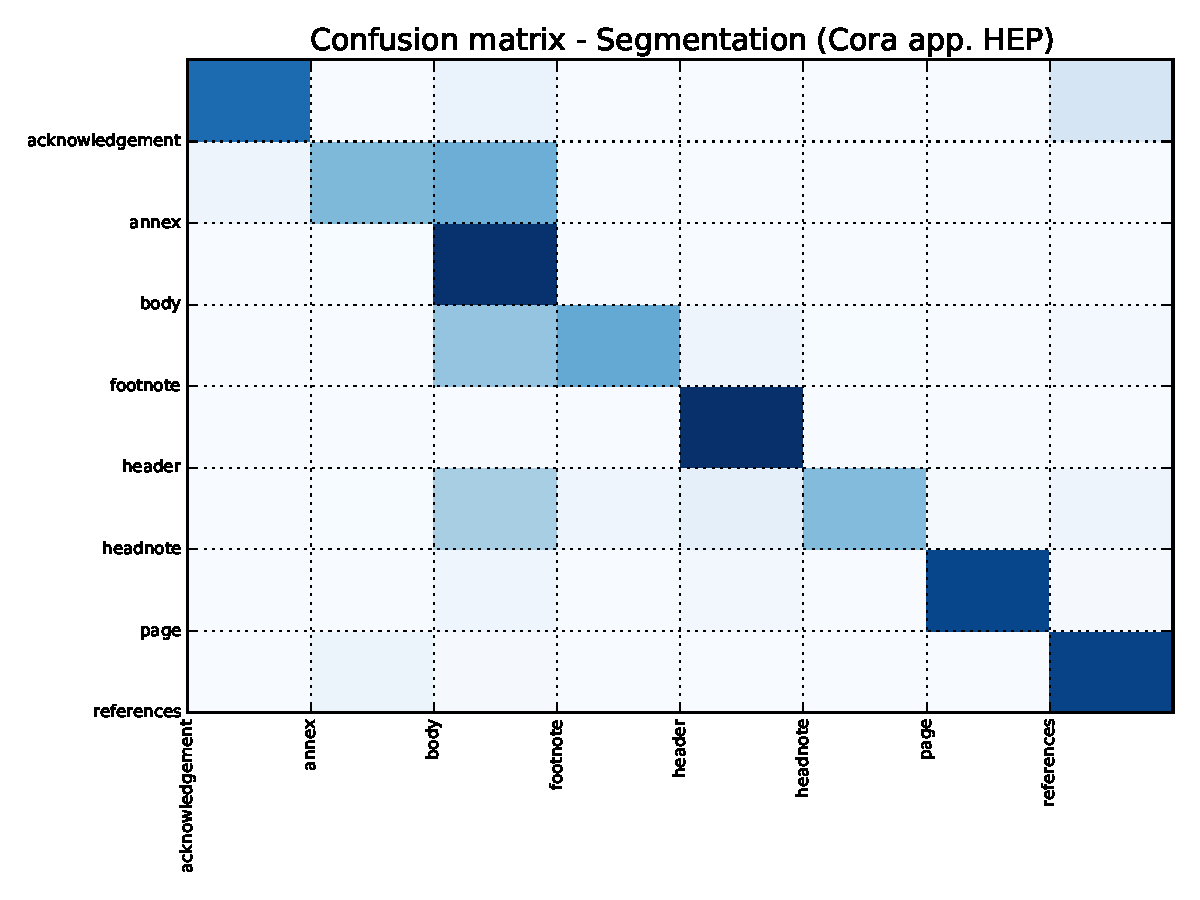
\includegraphics[width=6in]{figures/confusion.pdf}
%\caption{Heat map visualisation of the confusion matrix for the shipped segmentation model. The main diagonal shows the majority correctness of the model, Notably, classification for <body> gives a high true positive rate (TP) (observe the contrast in the <body> row), but a high number of false positives (observe the confusion in the <body> column), i.e. the false \emph{negatives} of other classes.}
%\label{fig:seg_confusion_1}
%\end{figure}

\end{document}